\documentclass[letterpaper
, superscriptaddress
, twocolumn
, aps
%, prl
%, showkeys
]{revtex4}

\usepackage[colorlinks=true,citecolor=blue,linkcolor=blue,pdfhighlight =/O]{hyperref}
\usepackage{graphicx}
\usepackage{amsmath}
\usepackage{mathtools}
%\usepackage{subcaption}
%\usepackage{epstopdf}
\usepackage{color}
\usepackage{soul}
\usepackage{natbib}
\usepackage{tikz} 

\bibliographystyle{apsrev4-1}
 
 %\usepackage[style=nature]{biblatex}
 
\hypersetup{urlcolor=blue}

\begin{document}

\title{Implementation of a Mathematical Model to Predict Radiotherapy Treatment Response of Non-Small Cell Lung Cancer Patients}

\author{R. Su}
\altaffiliation[]{On undergraduate co-op placement at Odette Cancer Centre, supervised by G. Pang from January 3 to May 1, 2020. Correspondance can be addressed to R. Su at \href{ruihengsu@alumni.ubc.ca}{ruihengsu@alumni.ubc.ca}}
\affiliation{Engineering Physics, The University of British Columbia, Vancouver, British Columbia V6T 1Z4, Canada}
\affiliation{Odette Cancer Centre, Ontario M4N 3M5, Canada}

\author{G. Pang}
%\altaffiliation[Also at ]{Physics Department, XYZ University.}
\affiliation{Department of Physics, Ryerson University, Toronto, Ontario M5B 2k3, Canada}
\affiliation{Odette Cancer Centre, Department of Radiation Oncology, University of Toronto, Ontario M4N 3M5, Canada}

\date{\today}

\begin{abstract}
We report on the development of a program that implements a mathematical model to describe radiation therapy treatment response of patients with non-small cell lung cancer proposed in an article by Geng et al. published in 2017. The program can predict the effect of well-separated radiation fractions on tumor growth and the Kaplan-Meier survival curve for an arbitrary patient population using a Monte Carlo method. While our program partially reproduces Geng et al.'s results well, further improvements to the source code and conceptual clarification is required.
\end{abstract}

\keywords{}

\maketitle

\section{Introduction}
Lung cancer is the leading cause of cancer-related deaths, and the most prevalent of all cancer types \cite{Bray2018}. While the 5-year relative survival rate of non-small cell lung cancer patients has improved by 8.7\% since 1975, it remains at 25.1\% as of 2015 \cite{Howlader19752016.November2018.April2019}. To increase the survival rate of cancer patients, clinicians can use mathematical modelling to optimize treatment scheduling and develop hypotheses for testing in clinical trials. 

While many papers have proposed new mathematical models for lung cancer, few describe the implementation of the models in detail. The goal of this paper is to illustrate our process to implement a program in \texttt{Python} based on a predictive model for non-small lung cancer growth and treatment response described in an article by Geng et al. published in 2017 \cite{Geng2017}. We also hope to provide some reasoning to the formulation of the mathematical model.

Non-small cell lung cancer accounts of 85\% of all lung cancer cases \cite{Molina2008}. It is less sensitive to chemotherapy and radiation therapy and takes longer to spread to other organs compared with small cell lung cancer \cite{PDQATEB2020}. 

Accurate cancer staging is important for both the clinician and the patient. Cancer staging is the process where clinician assigns a standardized metric to the state of growth and spread of the patient's tumor, which translates into the patient's prognostic information and eligibility for clinical trials. We will refer to the tumor, node, metastasis (TNM) staging system in this paper. The TNM system assesses the size of the primary tumor (T), the degree of lymph node involvement (N), and the presence or absence of metastasis (M) \cite{Tsim2010}. Once these three categories are assessed, a stage number of 0, I, II, III, and IV in an order of increasing severity is assigned to the patient.

The preferred treatment method for lung cancer is surgical resection \cite{Molina2008, PDQATEB2020}. The feasibility of surgical resection depends on whether the tumor remains at its primary site or has metastasized, and whether the patient can tolerate the surgery. Since patients are still at risk of relapse after surgery, additional chemotherapy and radiotherapy is used. For locally advanced unresectable tumors, which makes up 40\% of non-small cell lung cancer patients \cite{Geng2017}, combined chemotherapy and radiotherapy is used to extend patient survival. This mixed combination of different treatment methods is known as adjuvant therapy. 

Each patient responds to adjuvant therapy differently. If clinicians can accurately predict the effect of treatment for any patient, then they can develop treatment regimens that increase patient survival. Mathematical modelling hopes to fill this role.  

\section{Methods}

We encourage the reader to refer to the source code while reading this paper:
\begin{center}
	\href{https://github.com/sillyPhotons/NSCLC_Modelling}{github.com/sillyPhotons/NSCLC\_Modelling}
\end{center}

\subsection{Mathematical Modelling}

Geng et al. proposed an ordinary differential equation to model non-small cell lung cancer growth that states the instantaneous rate of change in the number of living tumor cells is the sum of three terms: the rate of constrained tumor growth; the effect of radiotherapy; the effect of chemotherapy. Each term of the equation includes multiple parameters that needs to be estimated before the equation can be solved. In this work, we will disregard the chemotherapy portion of the equation.

While Geng et al. state their equation in terms of tumor cell number, $N$, we will state them in terms of tumor volume, $V$. The two formulations differ only by a factor of tumor cell density.

\subsubsection{Constrained Tumor Growth}
The first term in the equation proposed describes constrained tumor growth.

Let $V(t)$ be the tumor volume a patient at time $t$ after diagnosis, $\rho$ be a patient specific tumor growth rate parameter 
%from an estimated univariate normal with mean $\rho_{\mu}$ and standard deviation $\rho_{\sigma}$
, and $K$ be the maximum tumor volume known as the carrying capacity. Geng et al. expects untreated tumor growth to follow Gompertzian kinetics - tumor growth rate decreases exponentially with time.
\begin{equation} \label{1}
\frac{dV(t)}{dt} = \rho V(t) \log \left( \frac{K}{V(t)}\right) \quad \text{Tumor Growth}
\end{equation}  

Given an initial tumor diameter, we can make the assumption of a spherical tumor to state the initial value problem,
\begin{equation*}
\frac{dV(t)}{dt} = \rho V(t) \log \left( \frac{K}{V(t)}\right) \qquad V(t_{0}) = V_{0}
\end{equation*}
Using the separation of variables,
\begin{equation*}
\begin{aligned}
&\int \frac{1}{V(t)} \left[\log \left(\frac{K}{V(t)}\right)\right]^{-1}\,dV(t) = \int \rho \, dt + C\\
&u = \log \left(\frac{K}{V(t)}\right) \,\,\, du =\frac{-1}{V}\,dV(t)\,\,\, \text{Apply $u$-substitution}
\end{aligned}
\end{equation*}
We obtain the analytic solution to equation \eqref{1}.
\begin{equation} \label{2}
V(t) = K \exp \left[- \log \left(\frac{K}{V_{0}}\right) e^{-\rho t} \right]
\end{equation}

\begin{figure}[b]
	\includegraphics[width=1.00\columnwidth]{Figures/fig1.pdf}
	\caption{Example plot of equation \eqref{2} and its derivative with $K = 1$, $\rho = 0.1$, $V_{0} = 0.1$. We observe that the inflection point occurs at $y = 1/e$ and $V(t)$ is asymmetric about its inflection point.}
	\label{eq2}
\end{figure} 

Examining equation \eqref{2}, in the limit as $t$ approaches infinity, the tumor volume, $V$, approaches the carrying capacity, $K$. This describes the clinically observed pattern of decreasing growth rate with increasing tumor size \cite{Geng2017, Grassberger2016, Benzekry2014}. Setting the second derivative of equation \eqref{2} to zero, we find that y-coordinate of the inflection point is precisely $K/e$, or $36.8\%$ of the carrying capacity. This makes equation \eqref{2} suitable for modelling processes that start to grow slower upon reaching approximately $1/3$ of its maximum size as seen in figure \ref{eq2}.

\subsubsection{Radiation Therapy Effect}
The second term in equation proposed describes the effect of radiotherapy on tumor growth.

Radiation therapy, or radiotherapy, is the use of focused ionizing radiation to kill tumor cells. High energy radiation causes the excitation of electrons at the tumor site through the photoelectric effect, Compton scattering, and pair production; producing free radicals that react with nearby molecules to induce chemical damage. The primary contribution to cell death is irreparable damage to DNA strands.

Historically, radiotherapy for non-small cell lung cancer is usually comprised of a total dose 60 to 70 Gy delivered using conventional fractionation - 1.8 to 2.0 Gy fractions per day \cite{PDQATEB2020}. Other fractionation schemes of clinical interest include hyperfractionation and accelerated fractionation \cite{Geng2017, PDQATEB2020}. Hyperfractionation involves the patient receiving a higher daily dose fraction, taking a shorter time to deliver the prescribed dose compared to conventional fractionation. Accelerated fractionation involves the patient receiving the same dose fraction as conventional fractionation, but more than once daily. 

The purpose of delivering radiation in separated fractions is to minimize harm to patients by allowing healthy cells time to repair. But having too much time between fractions can cause tumor cells to repopulate, decreasing the effectiveness of radiotherapy and increasing total dose needed to achieve the intended effect.
 
The most widely used model for radiation effect modelling is the linear-quadratic model \cite{Geng2017, Grassberger2016, Mayles2008, Brenner2008}, which is well validated from 1 to 10 Gy per fraction and can be used up to 18 Gy per fraction\cite{Brenner2008}. Below 1 Gy per fraction, some cells \textit{in vitro} and \textit{in vivo} display increased sensitivity to radiation (radiosensitivity), deviating from the linear-quadratic model \cite{Mayles2008}. 

Geng et al. used the linear-quadratic model to predict the effects radiation fractions to tumor cell growth, assuming all fractions are well-separated and instantaneously delivered. While the general form of the equation includes the Lea-Catcheside time factor in the quadratic dose term, the factor reduces to 1 under this assumption \cite{Brenner2008, Grassberger2016}.   

Let $\delta(t)$ be the Dirac delta function, $t_{R}$ be the time of radiation, $\alpha$ be a patient specific radiosensitivity parameter with units $\text{Gy}^{-1}$, $\beta$ be a constant with units $\text{Gy}^{-2}$, and $d$ be a constant representing the dose per fraction. The radiotherapy term is given by
\begin{equation} \label{3}
\frac{dV(t)}{dt} = - \delta(t - t_{R}) V(t)(\alpha d + \beta d^{2}) \quad \text{Radiotherapy}
\end{equation}
Geng et al. assumes that $\alpha / \beta = 10$ Gy for tumor tissues. 

%The tumor growth rate, $\rho$, and radiosensitivity, $\alpha$, are patient specific parameters. 
%As cells with faster growth rate have shown to be more sensitive to the harming effects of ionizing radiation \cite{Geng2017}, Geng et al. introduces a linear correlation coefficient, $\psi$, between $\alpha$ and $\rho$. By definition, $\psi$ is the ratio of the covariance of $\alpha$ and $\rho$ and the product of $\alpha_{\sigma}$ and $\rho_{\sigma}$.
%
%To draw correlated $(\alpha, \rho)$ samples, we pass an array $(\alpha_{\mu}, \rho_{\mu})$, and a covariance matrix $\mathbf{C}$, where
%\begin{equation*}
%\mathbf{C} = 
%\begin{bmatrix}
%\alpha_{\sigma}^{2} & \left(\alpha_{\sigma}\rho_{\sigma}\right)/\psi\\
%\left(\alpha_{\sigma}\rho_{\sigma}\right)/\psi & \rho_{\sigma}^{2}
%\end{bmatrix}
%\end{equation*}
%to the \texttt{multivariate\_normal} function of the \texttt{Numpy} library in \texttt{python}. 

Geng et al.'s original article did not contain the Dirac delta function, $\delta(t - t_{R})$ with units $\text{days}^{-1}$; equation \eqref{3} is the formulation given in a later correction \cite{Changran2018}. 

\subsubsection{Discrete-Time Model}

The sum of equation \eqref{1} and equation \eqref{3} results in Geng et al.'s model for the instantaneous rate of change in tumor volume of a non-small cell lung cancer patient treated with radiation therapy. 
\begin{equation}\label{4}
\frac{dV(t)}{dt} = \rho V(t) \log \left(\frac{K}{V(t)}\right) - \delta(t - t_{R}) V(t) (\alpha d + \beta d^{2})
\end{equation}

While Geng et al. solved equation \eqref{4} in \texttt{Python} using the \texttt{odeint} function of the \texttt{SciPy} library \cite{Changran2018}, we solved equation \eqref{4} via time stepping using discrete-time models.

But there is one problem. Equation \eqref{4} cannot be evaluated in its current form due to the Dirac delta function, which is undefined at the point of impulse, $t_{R}$. 

We propose a formulation without the delta function. For $n$ dose fractions delivered at times $t_{1}, \dots, t_{n}$, let $\delta_{t,t_{R}}$ be the Kronecker delta function, where 
\begin{equation*}
	\delta_{t, t_{R}} = 
\begin{cases*}
&1 \quad \text{when $t = t_{R}$}\\
&0 \quad \text{when $t \not = t_{R}$}
\end{cases*}
\end{equation*}
We define a function, $D(t)$, where
\begin{equation}
D(t) = d \sum_{R = 1}^{n} \delta_{t, t_{R}}
\end{equation}

We will use the following redefinition of equation \eqref{4} for the remainder of this paper.
\begin{equation} \label{dv/dt}
\frac{dV(t)}{dt} = \rho V(t) \log \left(\frac{K}{V(t)}\right) - V(t) \left(\alpha D(t) + \beta D(t)^{2}\right)
\end{equation}
\begin{figure*}
	\centering
	
	\tikzset{every picture/.style={line width=0.75pt}} %set default line width to 0.75pt        
	
	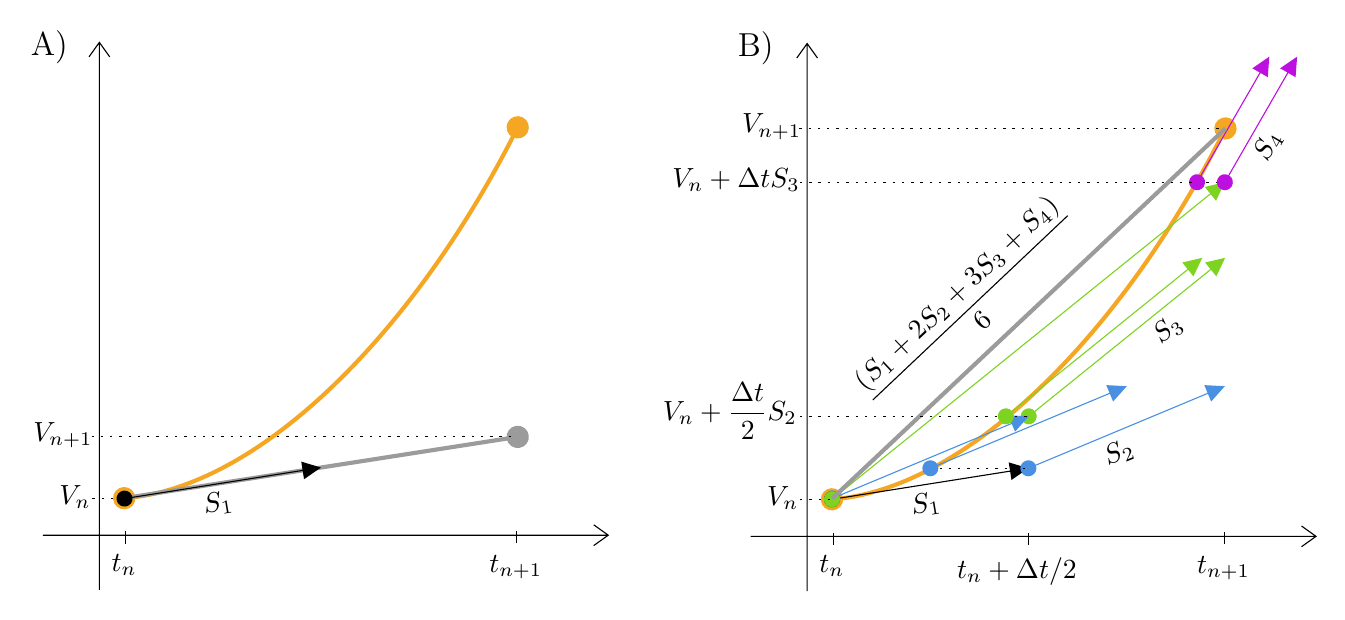
\begin{tikzpicture}[x=0.75pt,y=0.75pt,yscale=-1,xscale=1]
	%uncomment if require: \path (0,300); %set diagram left start at 0, and has height of 300
	
	%Shape: Axis 2D [id:dp0771007287176293] 
	\draw  (29.7,250.86) -- (302.12,250.86)(56.94,13.42) -- (56.94,277.24) (295.12,245.86) -- (302.12,250.86) -- (295.12,255.86) (51.94,20.42) -- (56.94,13.42) -- (61.94,20.42)  ;
	%Curve Lines [id:da08434347737765924] 
	\draw [color={rgb, 255:red, 245; green, 166; blue, 35 }  ,draw opacity=1 ][line width=1.5]    (68.91,233.02) .. controls (133.63,228.38) and (208.74,153.51) .. (258.5,54.35) ;
	\draw [shift={(258.5,54.35)}, rotate = 296.65] [color={rgb, 255:red, 245; green, 166; blue, 35 }  ,draw opacity=1 ][fill={rgb, 255:red, 245; green, 166; blue, 35 }  ,fill opacity=1 ][line width=1.5]      (0, 0) circle [x radius= 4.36, y radius= 4.36]   ;
	\draw [shift={(68.91,233.02)}, rotate = 355.9] [color={rgb, 255:red, 245; green, 166; blue, 35 }  ,draw opacity=1 ][fill={rgb, 255:red, 245; green, 166; blue, 35 }  ,fill opacity=1 ][line width=1.5]      (0, 0) circle [x radius= 4.36, y radius= 4.36]   ;
	%Straight Lines [id:da34948866688298375] 
	\draw    (258.03,248.84) -- (258.03,254.43) ;
	%Straight Lines [id:da052581047783268886] 
	\draw    (69.52,248.84) -- (69.52,254.91) ;
	%Straight Lines [id:da38723286729247786] 
	\draw  [dash pattern={on 0.84pt off 2.51pt}]  (53.56,233.02) -- (68.91,233.02) ;
	%Shape: Axis 2D [id:dp38547510778353544] 
	\draw  (370.7,251.41) -- (643.12,251.41)(397.94,13.97) -- (397.94,277.79) (636.12,246.41) -- (643.12,251.41) -- (636.12,256.41) (392.94,20.97) -- (397.94,13.97) -- (402.94,20.97)  ;
	%Curve Lines [id:da17073823988745307] 
	\draw [color={rgb, 255:red, 245; green, 166; blue, 35 }  ,draw opacity=1 ][line width=1.5]    (409.91,233.57) .. controls (474.63,228.94) and (549.74,154.06) .. (599.5,54.9) ;
	\draw [shift={(599.5,54.9)}, rotate = 296.65] [color={rgb, 255:red, 245; green, 166; blue, 35 }  ,draw opacity=1 ][fill={rgb, 255:red, 245; green, 166; blue, 35 }  ,fill opacity=1 ][line width=1.5]      (0, 0) circle [x radius= 4.36, y radius= 4.36]   ;
	\draw [shift={(409.91,233.57)}, rotate = 355.9] [color={rgb, 255:red, 245; green, 166; blue, 35 }  ,draw opacity=1 ][fill={rgb, 255:red, 245; green, 166; blue, 35 }  ,fill opacity=1 ][line width=1.5]      (0, 0) circle [x radius= 4.36, y radius= 4.36]   ;
	%Straight Lines [id:da7010678026762633] 
	\draw    (409.91,233.57) -- (501.58,219.07) ;
	\draw [shift={(504.55,218.61)}, rotate = 531.02] [fill={rgb, 255:red, 0; green, 0; blue, 0 }  ][line width=0.08]  [draw opacity=0] (8.93,-4.29) -- (0,0) -- (8.93,4.29) -- cycle    ;
	\draw [shift={(409.91,233.57)}, rotate = 351.02] [color={rgb, 255:red, 0; green, 0; blue, 0 }  ][fill={rgb, 255:red, 0; green, 0; blue, 0 }  ][line width=0.75]      (0, 0) circle [x radius= 3.35, y radius= 3.35]   ;
	%Straight Lines [id:da7913384624553639] 
	\draw    (504.55,249.87) -- (504.55,255.46) ;
	%Straight Lines [id:da23481194682569373] 
	\draw [color={rgb, 255:red, 74; green, 144; blue, 226 }  ,draw opacity=1 ]   (504.55,218.61) -- (596.42,180.23) ;
	\draw [shift={(599.19,179.07)}, rotate = 517.3299999999999] [fill={rgb, 255:red, 74; green, 144; blue, 226 }  ,fill opacity=1 ][line width=0.08]  [draw opacity=0] (8.93,-4.29) -- (0,0) -- (8.93,4.29) -- cycle    ;
	\draw [shift={(504.55,218.61)}, rotate = 337.33] [color={rgb, 255:red, 74; green, 144; blue, 226 }  ,draw opacity=1 ][fill={rgb, 255:red, 74; green, 144; blue, 226 }  ,fill opacity=1 ][line width=0.75]      (0, 0) circle [x radius= 3.35, y radius= 3.35]   ;
	%Straight Lines [id:da301545945803672] 
	\draw [color={rgb, 255:red, 126; green, 211; blue, 33 }  ,draw opacity=1 ][fill={rgb, 255:red, 255; green, 255; blue, 255 }  ,fill opacity=1 ]   (504.7,193.59) -- (597.01,119.09) ;
	\draw [shift={(599.34,117.21)}, rotate = 501.09] [fill={rgb, 255:red, 126; green, 211; blue, 33 }  ,fill opacity=1 ][line width=0.08]  [draw opacity=0] (8.93,-4.29) -- (0,0) -- (8.93,4.29) -- cycle    ;
	\draw [shift={(504.7,193.59)}, rotate = 321.09] [color={rgb, 255:red, 126; green, 211; blue, 33 }  ,draw opacity=1 ][fill={rgb, 255:red, 126; green, 211; blue, 33 }  ,fill opacity=1 ][line width=0.75]      (0, 0) circle [x radius= 3.35, y radius= 3.35]   ;
	%Straight Lines [id:da4511439811043032] 
	\draw  [dash pattern={on 0.84pt off 2.51pt}]  (457.31,218.61) -- (504.55,218.61) ;
	%Straight Lines [id:da20626819623032833] 
	\draw [color={rgb, 255:red, 74; green, 144; blue, 226 }  ,draw opacity=1 ]   (410.07,233.12) -- (501.94,194.75) ;
	\draw [shift={(504.7,193.59)}, rotate = 517.3299999999999] [fill={rgb, 255:red, 74; green, 144; blue, 226 }  ,fill opacity=1 ][line width=0.08]  [draw opacity=0] (8.93,-4.29) -- (0,0) -- (8.93,4.29) -- cycle    ;
	\draw [shift={(410.07,233.12)}, rotate = 337.33] [color={rgb, 255:red, 74; green, 144; blue, 226 }  ,draw opacity=1 ][fill={rgb, 255:red, 74; green, 144; blue, 226 }  ,fill opacity=1 ][line width=0.75]      (0, 0) circle [x radius= 3.35, y radius= 3.35]   ;
	%Straight Lines [id:da36208750075131446] 
	\draw [color={rgb, 255:red, 74; green, 144; blue, 226 }  ,draw opacity=1 ]   (457.31,218.61) -- (549.18,180.23) ;
	\draw [shift={(551.95,179.07)}, rotate = 517.3299999999999] [fill={rgb, 255:red, 74; green, 144; blue, 226 }  ,fill opacity=1 ][line width=0.08]  [draw opacity=0] (8.93,-4.29) -- (0,0) -- (8.93,4.29) -- cycle    ;
	\draw [shift={(457.31,218.61)}, rotate = 337.33] [color={rgb, 255:red, 74; green, 144; blue, 226 }  ,draw opacity=1 ][fill={rgb, 255:red, 74; green, 144; blue, 226 }  ,fill opacity=1 ][line width=0.75]      (0, 0) circle [x radius= 3.35, y radius= 3.35]   ;
	%Straight Lines [id:da7349482571473773] 
	\draw  [dash pattern={on 0.84pt off 2.51pt}]  (493.68,193.59) -- (504.7,193.59) ;
	%Straight Lines [id:da35414907068052437] 
	\draw [color={rgb, 255:red, 126; green, 211; blue, 33 }  ,draw opacity=1 ][fill={rgb, 255:red, 255; green, 255; blue, 255 }  ,fill opacity=1 ]   (409.91,233.57) -- (596.85,82.69) ;
	\draw [shift={(599.19,80.8)}, rotate = 501.09] [fill={rgb, 255:red, 126; green, 211; blue, 33 }  ,fill opacity=1 ][line width=0.08]  [draw opacity=0] (8.93,-4.29) -- (0,0) -- (8.93,4.29) -- cycle    ;
	\draw [shift={(409.91,233.57)}, rotate = 321.09] [color={rgb, 255:red, 126; green, 211; blue, 33 }  ,draw opacity=1 ][fill={rgb, 255:red, 126; green, 211; blue, 33 }  ,fill opacity=1 ][line width=0.75]      (0, 0) circle [x radius= 3.35, y radius= 3.35]   ;
	%Straight Lines [id:da043396702764612716] 
	\draw  [dash pattern={on 0.84pt off 2.51pt}]  (585.8,80.8) -- (599.19,80.8) ;
	%Straight Lines [id:da32188701807638465] 
	\draw [color={rgb, 255:red, 189; green, 16; blue, 224 }  ,draw opacity=1 ][fill={rgb, 255:red, 255; green, 255; blue, 255 }  ,fill opacity=1 ]   (585.8,80.8) -- (619.13,22.91) ;
	\draw [shift={(620.62,20.31)}, rotate = 479.93] [fill={rgb, 255:red, 189; green, 16; blue, 224 }  ,fill opacity=1 ][line width=0.08]  [draw opacity=0] (8.93,-4.29) -- (0,0) -- (8.93,4.29) -- cycle    ;
	\draw [shift={(585.8,80.8)}, rotate = 299.93] [color={rgb, 255:red, 189; green, 16; blue, 224 }  ,draw opacity=1 ][fill={rgb, 255:red, 189; green, 16; blue, 224 }  ,fill opacity=1 ][line width=0.75]      (0, 0) circle [x radius= 3.35, y radius= 3.35]   ;
	%Straight Lines [id:da2615827450281447] 
	\draw [color={rgb, 255:red, 189; green, 16; blue, 224 }  ,draw opacity=1 ][fill={rgb, 255:red, 255; green, 255; blue, 255 }  ,fill opacity=1 ]   (599.19,80.8) -- (632.51,22.91) ;
	\draw [shift={(634.01,20.31)}, rotate = 479.93] [fill={rgb, 255:red, 189; green, 16; blue, 224 }  ,fill opacity=1 ][line width=0.08]  [draw opacity=0] (8.93,-4.29) -- (0,0) -- (8.93,4.29) -- cycle    ;
	\draw [shift={(599.19,80.8)}, rotate = 299.93] [color={rgb, 255:red, 189; green, 16; blue, 224 }  ,draw opacity=1 ][fill={rgb, 255:red, 189; green, 16; blue, 224 }  ,fill opacity=1 ][line width=0.75]      (0, 0) circle [x radius= 3.35, y radius= 3.35]   ;
	%Straight Lines [id:da8599095105658559] 
	\draw [color={rgb, 255:red, 126; green, 211; blue, 33 }  ,draw opacity=1 ][fill={rgb, 255:red, 255; green, 255; blue, 255 }  ,fill opacity=1 ]   (493.68,193.59) -- (585.99,119.09) ;
	\draw [shift={(588.32,117.21)}, rotate = 501.09] [fill={rgb, 255:red, 126; green, 211; blue, 33 }  ,fill opacity=1 ][line width=0.08]  [draw opacity=0] (8.93,-4.29) -- (0,0) -- (8.93,4.29) -- cycle    ;
	\draw [shift={(493.68,193.59)}, rotate = 321.09] [color={rgb, 255:red, 126; green, 211; blue, 33 }  ,draw opacity=1 ][fill={rgb, 255:red, 126; green, 211; blue, 33 }  ,fill opacity=1 ][line width=0.75]      (0, 0) circle [x radius= 3.35, y radius= 3.35]   ;
	%Straight Lines [id:da6725603579410842] 
	\draw [color={rgb, 255:red, 155; green, 155; blue, 155 }  ,draw opacity=1 ][fill={rgb, 255:red, 255; green, 255; blue, 255 }  ,fill opacity=1 ][line width=1.5]    (410.07,233.12) -- (599.5,54.9) ;
	%Straight Lines [id:da5130940616762998] 
	\draw    (599.03,249.39) -- (599.03,254.98) ;
	%Straight Lines [id:da44175903423776663] 
	\draw    (410.52,249.87) -- (410.52,255.46) ;
	%Straight Lines [id:da44303959754743527] 
	\draw  [dash pattern={on 0.84pt off 2.51pt}]  (394.48,80.8) -- (585.8,80.8) ;
	%Straight Lines [id:da5269258649069042] 
	\draw  [dash pattern={on 0.84pt off 2.51pt}]  (394.46,193.59) -- (491.79,193.59) ;
	%Straight Lines [id:da5550613969524896] 
	\draw  [dash pattern={on 0.84pt off 2.51pt}]  (394.14,54.9) -- (599.5,54.9) ;
	%Straight Lines [id:da38028364332852105] 
	\draw  [dash pattern={on 0.84pt off 2.51pt}]  (394.56,233.57) -- (409.91,233.57) ;
	%Straight Lines [id:da9901136897520815] 
	\draw [color={rgb, 255:red, 155; green, 155; blue, 155 }  ,draw opacity=1 ][fill={rgb, 255:red, 255; green, 255; blue, 255 }  ,fill opacity=1 ][line width=1.5]    (68.91,233.02) -- (258.5,203.49) ;
	\draw [shift={(258.5,203.49)}, rotate = 351.15] [color={rgb, 255:red, 155; green, 155; blue, 155 }  ,draw opacity=1 ][fill={rgb, 255:red, 155; green, 155; blue, 155 }  ,fill opacity=1 ][line width=1.5]      (0, 0) circle [x radius= 4.36, y radius= 4.36]   ;
	%Straight Lines [id:da9871797977090848] 
	\draw  [dash pattern={on 0.84pt off 2.51pt}]  (53.17,203.49) -- (258.5,203.49) ;
	%Straight Lines [id:da3540438836431492] 
	\draw    (69.07,233.22) -- (160.74,218.72) ;
	\draw [shift={(163.7,218.26)}, rotate = 531.02] [fill={rgb, 255:red, 0; green, 0; blue, 0 }  ][line width=0.08]  [draw opacity=0] (8.93,-4.29) -- (0,0) -- (8.93,4.29) -- cycle    ;
	\draw [shift={(69.07,233.22)}, rotate = 351.02] [color={rgb, 255:red, 0; green, 0; blue, 0 }  ][fill={rgb, 255:red, 0; green, 0; blue, 0 }  ][line width=0.75]      (0, 0) circle [x radius= 3.35, y radius= 3.35]   ;
	
	% Text Node
	\draw (104.8,230.26) node [anchor=north west][inner sep=0.75pt]  [rotate=-350.52] [align=left] {$\displaystyle S_{1}$};
	% Text Node
	\draw (23.87,195.26) node [anchor=north west][inner sep=0.75pt]   [align=left] {$\displaystyle V_{n+1}$};
	% Text Node
	\draw (243.53,259.31) node [anchor=north west][inner sep=0.75pt]   [align=left] {$\displaystyle t_{n+1}$};
	% Text Node
	\draw (61.57,258.67) node [anchor=north west][inner sep=0.75pt]   [align=left] {$\displaystyle t_{n}$};
	% Text Node
	\draw (36.42,225.79) node [anchor=north west][inner sep=0.75pt]   [align=left] {$\displaystyle V_{n}$};
	% Text Node
	\draw (468.94,260.42) node [anchor=north west][inner sep=0.75pt]   [align=left] {$\displaystyle t_{n} +\Delta t /2$};
	% Text Node
	\draw (445.8,230.81) node [anchor=north west][inner sep=0.75pt]  [rotate=-350.52] [align=left] {$\displaystyle S_{1}$};
	% Text Node
	\draw (537.88,207.97) node [anchor=north west][inner sep=0.75pt]  [rotate=-338.28] [align=left] {$\displaystyle S_{2}$};
	% Text Node
	\draw (560.99,151.81) node [anchor=north west][inner sep=0.75pt]  [rotate=-321.85] [align=left] {$\displaystyle S_{3}$};
	% Text Node
	\draw (609.95,67.24) node [anchor=north west][inner sep=0.75pt]  [rotate=-299.99] [align=left] {$\displaystyle S_{4}$};
	% Text Node
	\draw (365.37,46.67) node [anchor=north west][inner sep=0.75pt]   [align=left] {$\displaystyle V_{n+1}$};
	% Text Node
	\draw (415.88,175.34) node [anchor=north west][inner sep=0.75pt]  [rotate=-316.6] [align=left] {$\displaystyle \frac{( S_{1} +2S_{2} +3S_{3} +S_{4})}{6}$};
	% Text Node
	\draw (584.53,259.86) node [anchor=north west][inner sep=0.75pt]   [align=left] {$\displaystyle t_{n+1}$};
	% Text Node
	\draw (402.57,259.22) node [anchor=north west][inner sep=0.75pt]   [align=left] {$\displaystyle t_{n}$};
	% Text Node
	\draw (327.14,176.19) node [anchor=north west][inner sep=0.75pt]   [align=left] {$\displaystyle V_{n} +\frac{\Delta t}{2} S_{2}$};
	% Text Node
	\draw (331.73,72.84) node [anchor=north west][inner sep=0.75pt]   [align=left] {$\displaystyle V_{n} +\Delta t S_{3}$};
	% Text Node
	\draw (377.42,226.34) node [anchor=north west][inner sep=0.75pt]   [align=left] {$\displaystyle V_{n}$};
	% Text Node
	\draw (22.67,6.6) node [anchor=north west][inner sep=0.75pt]  [font=\large] [align=left] {A)};
	% Text Node
	\draw (363.33,6.92) node [anchor=north west][inner sep=0.75pt]  [font=\large] [align=left] {B)};
	
	
	\end{tikzpicture}
	
	\caption{A): One time step of the forward Euler's method. B): One time step of of the fourth order Runge-Kutta method. The grey line has a slope equal to the weighted average of $S_{1}, S_{2}, S_{3}, S_{4}$. The black arrow has slope $S_{1}$. The blue arrows have slope $S_{2}$. The green arrows have slope $S_{3}$. The purple arrows have slope $S_{4}$. A single step using the fourth order Runge-Kutta method can be much more accurate than the forward Euler's method, but requires more function evaluations.}
	\label{discrete}
	
\end{figure*}

Given the initial tumor volume, $V_{0}$, and the values of $\rho, K, \alpha, \beta,$ and $d$, the simplest discrete-time mode we can formulate is based on the forward Euler's method, relying on successive linear approximations. Let $dV(t)/dt = f(t,V)$, and $\Delta t$ be the step size, the model is given by
\begin{equation}\label{5}
V_{n + 1} = f(t_{n}, V_{n}) \Delta t + V_{n}
\end{equation}

The forward Euler's method model only requires a single function evaluation per time step. But it lacks in accuracy for non-smooth functions or when the step size $\Delta t$ is too large. It can be shown that the forward Euler's method is a first order method - halving step size reduces the error by a factor of 2. Figure \ref{discrete}A visualizes a single time step using the forward Euler's method.

We implemented another model based on the fourth order Runge-Kutta method, which offers better accuracy (halving step size reduces error by factor of $2^{4}$) at the price of requiring four function evaluations per time step. Let $dV/dt = f(t, V)$, then
\begin{equation}\label{6}
\begin{aligned}
S_{1} &= f(t_{n}, V_{n})\\
S_{2} &= f(t_{n} + \frac{\Delta t}{2}, V_{n} + \Delta t\frac{S_{1}}{2})\\
S_{3} &= f(t_{n} + \frac{\Delta t}{2}, V_{n} + \Delta t\frac{S_{2}}{2})\\
S_{4} &= f(t_{n} + \Delta t, V_{n} + \Delta t S_{3})\\
V_{n + 1} &= V_{n} + \frac{\Delta t}{6} (S_{1} + 2S_{2} + 2S_{3} + S_{4})
\end{aligned}
\end{equation}
We visualized a single time step of this model in figure \ref{discrete}B. We can see the difference in accuracy between the forward Euler's method model and the Runge-Kutta method model by comparing A and B of figure \ref{discrete}. 

The final discrete-time model we implemented was used by Geng et al., involving an exponential \cite{Changran2018}.
\begin{equation}\label{7}
V_{n + 1} = V_{n} e^{\rho \Delta t \log \left( \frac{K}{V_{n}} \right) - (\alpha D(t) + \beta D(t)^{2})}
\end{equation}

% We have given the mathematical definitions of the discrete-time models used to solve equation \eqref{dv/dt}. In the following section, we will explain the process to obtain numerical values for $\rho, K, \alpha$ and the correlation coefficient $\psi$ between $\rho$ and $\alpha$.

\begin{table*}
	\includegraphics[scale=0.3]{Figures/table.png}
	\caption{Summary of required parameters to solve the tumor growth model radiotherapy treatment effect for a single patient. The constraints for the volume distributions are given in terms of diameter. In the actual implementation, samples of a tumor diameter distribution is converted to volume by assuming a spherical tumor. Geng et al. assume the minimum detectable tumor diameter is $0.3$ cm.}
	\label{table1}
\end{table*}

\subsection{Parameter Estimation}

Since the parameters $\rho$ and $\alpha$ are patient specific - we expect their values to vary from patient to patient - a reasonable assumption to make is that $\alpha$ and $\rho$ value are normally distributed across all patients.

To acquire values for $\rho$ and $\alpha$ requires estimating the mean and standard deviation of their normal distributions. But as cells with faster growth rate have shown to be more sensitive to the harming effects of ionizing radiation \cite{Geng2017}, a linear correlation coefficient, $\psi$, between the distributions of $\alpha$ and $\rho$ can be introduced. Let $\alpha_{\mu}$, $\rho_{\mu}$ be the mean and $\alpha_{\sigma}$, $\rho_{\sigma}$, be the standard deviation of $\alpha$ and $\rho$ distributions. By definition, $\psi$ is the ratio of the covariance of $\alpha$ and $\rho$ and the product of $\alpha_{\sigma}$ and $\rho_{\sigma}$.

To draw correlated $(\alpha, \rho)$ samples, we pass an array $(\alpha_{\mu}, \rho_{\mu})$, and a covariance matrix $\mathbf{C}$, where
\begin{equation*}
\mathbf{C} = 
\begin{bmatrix}
\alpha_{\sigma}^{2} & \left(\alpha_{\sigma}\rho_{\sigma}\right)/\psi\\
\left(\alpha_{\sigma}\rho_{\sigma}\right)/\psi & \rho_{\sigma}^{2}
\end{bmatrix}
\end{equation*}
to the \texttt{multivariate\_normal} function of the \texttt{Numpy} library in \texttt{Python}. 

Similarly, we can interpret the initial tumor diameter for a patient to be a sample from the diameter distribution of the stage that the patient belongs in. From clinical observations, Geng et al. assume these distribution are log-normal distributions. 

To obtain a value for the initial tumor diameter for an arbitrary patient in a specific cancer stage then requires estimating the diameter distribution for that stage. A tumor volume can be specified by the tumor diameter, assuming a spherical tumor. We specified the log-normal tumor volume distribution for each cancer stage by the mean, $V_{\mu}^{\text{I,\dots,IV}}$, and the standard deviation, $V_{\sigma}^{\text{I,\dots,IV}}$ its underlying normal distribution in terms of tumor diameter.

The parameter estimation process involves fitting clinical data to obtain estimates for $\rho_{\mu}$, $\rho_{\sigma}$, $K$, $\alpha_{\mu}$, $\alpha_{\sigma}$, $\psi$, $V^{\text{I,\dots,IV}}_{\mu}$, and $V^{\text{I,\dots,IV}}_{\sigma}$ for a total of 16 parameters.

Geng et al. fit Kaplan-Meier survival curves generated using a Monte Carlo method based on equation \eqref{dv/dt} to clinical survival curves obtained from the California Cancer Registry \cite{Raz2007}, and the RTOG-8808 clinical trial \cite{Sause2001}. 

The California Cancer Registry data set contains survival curves of 22945 (Geng et al. mistakenly cites 23954 patients) untreated stage I, II, IIIA, IIIB, and IV non-small cell lung cancer patients. The RTOG-8808 trial data set contains the survival curve of a population of 9 stage I, 67 stage IIIA, and 76 stage IIIB patients that received conventional radiotherapy with 2 Gy fractions for 5 days a week to 60 Gy. But since these data sets were inaccessible during this project, we used an online data extraction tool (\texttt{WebPlotDigitizer}) \cite{Marin2017} to estimate the data  - spanning 59 months after diagnosis - from figures 3 and 5 from Geng et al.'s paper instead. The survival curves from the two data sets are shown in figures \ref{untreated} and \ref{rad}.

\begin{figure}[h]
	\includegraphics[width=1.00\columnwidth]{Figures/untreated_data.pdf}
	\caption{Plot of the survival curves for untreated non-small cell lung cancer patients estimated from figure 3 of Geng et al.'s paper. We can see that the initial slopes of the curve increases in magnitude with cancer stage.}
	\label{untreated}
\end{figure}

\begin{figure}[h]
	\includegraphics[width=1.00\columnwidth]{Figures/rad_data.pdf}
	\caption{Plot of the survival curve for non-small cell lung cancer patients from the standard radiotherapy arm in the RTOG-8808 clinical trial estimated from figure 5 of Geng et al.'s paper.}
	\label{rad} 
\end{figure}

\begin{figure*}
	\centering
	\includegraphics[scale=0.27]{Figures/param_estimation.png}
	\caption{In step 1, Geng et al. optimized the tumor growth parameters using survival curves of untreated patients and pre-defined volume distributions for each stage. Geng et al. then optimized the volume distributions for each stage using the optimized tumor growth parameters. In step 2, Geng et al. optimized the radiosensitivity parameter, $\alpha$, by replicating the patient population and radiotherapy fractionation used by the standard radiotherapy arm of the RTOG-8808 trial, and assuming that $\alpha/\beta = 10$. Geng et al. optimized the linear correlation coefficient between $\alpha$ and $\rho$ last, holding all optimized parameters constant.}
	\label{param_estimation}
\end{figure*}
\begin{figure*}
	\centering
	\includegraphics[scale=0.26]{Figures/kaplan_mini.png}
	\caption{A): The parameter optimization process. The \texttt{minimize} function recursively explores the parameter space using Powell's method. B): The Kaplan-Meier survival curve generation process. The key assumption of is that the patient is dies when the tumor diameter exceeds 13 cm. While Geng et al. defines the death condition in terms of diameter, the program converts this to tumor volume, assuming a spherical tumor.}
	\label{kaplan_mini}
\end{figure*}

\subsubsection{Parameter Optimization}

Since a 16-dimensional parameter space cannot be efficiently searched, Geng et al. proposed a multi-stepped estimation process, as shown in figure \ref{param_estimation}.

Geng et al. define the cost function for minimization as the of sum of the variance between a survival curve from clinical data and a survival curve generated from our discrete-time model using a Monte-Carlo method. We used the \texttt{minimize} function from the \texttt{lmfit} library \cite{Newville2014} to automate the minimization process shown in figure \ref{kaplan_mini}A using Powell's method.

In \texttt{Python}, we define our cost function to take: a variable number of parameters; $x$- and $y$-coordinates arrays of the survival curve data; a function object that implements one of three discrete-time model described (functions are objects in \texttt{Python}). As opposed to returning a sum of residuals as done by Geng et al., our cost function returns an array of residuals between the model and data to be minimized, as required by the \texttt{lmfit} documentation. Let $\mathbf{SF}$ be a $1$ by $n$ vector, where $n$ corresponds to the number of time steps between the initial and final time of the simulated time interval, and the $i^{th}$ element represents the proportion of patients alive after $i$ time steps. Our cost function maps the values of a set of parameter values to a vector of residuals between $\mathbf{SF}$ of the model and data.
\begin{equation} 
\mathbf{SF}_{\text{model}} - \mathbf{SF}_{\text{data}}
\end{equation}

\subsubsection{Monte Carlo Patient Population}

Figure \ref{kaplan_mini}A shows that parameter optimization requires generating a Monte Carlo patient population to replicate the initial tumor characteristics of patients in the data. The parameters we generate for each patient is summarized in table \ref{table1}. 

\begin{table*}
	\includegraphics[scale=0.3]{Figures/table2.png}
	\caption{Summary of the numerical parameter values used to reproduce Geng et al.'s results. We source these values from: tables 3 and 2, and page 1 of Geng et al.'s paper; and the description of the standard radiotherapy arm in Sause et al.'s paper on the RTOG-8808 trial.}
	\label{table2}
\end{table*}

\subsubsection{Kaplan-Meier Survival Curve Generation}
The procedure to generate a Kaplan-Meier survival curve is shown in figure \ref{kaplan_mini}B. After generating Monte Carlo patient population and specifying magnitude of each time step in units of days, we use a discrete-time model to observe the tumor growth for each patient in the population. Following each time step, we check whether the current tumor diameter exceeds the death diameter followed by whether the patient recovers.

For consistency with Geng et al.'s work, we used a step size of $\Delta t = 0.01$ days, and 10000 patients per Monte Carlo population \cite{Changran2018}. But such a fine step size and large number of patients can cause a significant increase in run-time for a sequential implementation, as the discrete time model must be evolved over the simulation interval for every patient. 

Our implementation highlights the power of parallel programming to reduce run-time. There are numerous options for parallelism in \texttt{Python} (e.g. \texttt{threading}, \texttt{multiprocessing}), but most are syntactically difficult to use. 

The \texttt{ray} library \cite{Moritz2017} offers a simple and scalable method to enable python functions to be run in parallel. Using \texttt{ray}, our program can solve the discrete-time model for multiple patients at a time during in each parameter optimization iteration. 

\subsection{Code Verification}

We applied test-driven development to minimize syntactic and conceptual errors. We ensured that the specifications of each function or class is met prior to run-time through unit tests written using the \texttt{unittest} library. 

We reasoned that our program is conceptually correct if the following conditions were met: parameters estimated using reported parameter values in Geng et al.'s paper as initial guesses, with a step size $> 0.01$ days and at least 1000 patients per Monte Carlo population does not deviate from the initial value by over 15\%; replications of figures 3, 4A, 5B, 6B in Geng et al.'s paper have negligible difference upon visual inspection.

To reproduce Geng et al.'s results, we used the parameter values reported in tables 2 and 3 of their paper for our program: table 2 gives the optimized mean and median of the log-normal volume distributions for each cancer stage in columns 3 and 4; table 3 gives the patient death diameter and optimized $\rho_{\mu}$, $\rho_{\sigma}$, $\alpha_{\mu}$, $\alpha_{\sigma}$, $K$, and $\psi$. Table 3 also provides some numerical values on the volume distributions of each stage. But the exact meaning of these values were not clearly stated. We found that survival curves generated by assuming that these values referred to $V_{\mu}^{\text{I,\dots,IV}}, V_{\sigma}^{\text{I,\dots,IV}}$ did not match the data for untreated patients. We believe values given table 1 and 3 refers to the underlying normal distribution while table 2 refers to actual log-normal distribution - this remains to be verified. 

The mean and median of a log-normal are related to the mean and standard deviation of its underlying normal distribution ($\mu, \sigma$) by the following equalities:
\begin{align*}
\mu &= \log \left( \text{median} \right)\\
\sigma &= \sqrt{2 | \log(\text{mean}) - \mu) |}
\end{align*}


We summarize the numerical values used for prediction in table \ref{table2}.

\subsection{Model Prediction}

After verifying the correctness of our program, we can use it to predict the Kaplan-Meier survival curve of a non-small cell lung cancer population made of stage I, II, IIIA, IIIB, and IV patients in user-defined proportions, or to simulate the effect of well-separated radiation fractions on tumor growth for a single patient.

\section{Results}
We verify the ability of our model to estimate parameter values, reproduce plots, and predict radiotherapy treatment response.

\subsection{Parameter Estimation}
We were unable the follow the complete parameter estimation process outlined in figure \ref{param_estimation} when each optimization is configured to use a 10000 patient population and a step size $\Delta t= 0.01$ days. This is because of a lack of virtual memory in the quad-core computer used, as the current program creates multiple large 2-dimensional arrays whose number of elements is proportional to the number of patients and inversely proportional to the step size. But even if the lack of memory is not an issue, we expect a lengthy run-time as the device used can only handle four tasks in parallel.

We argued that our model's ability to estimate parameters can be demonstrated if setting initial guesses to reported values does not deviate from the reported value by more than 15\% for a simulated population of $\leq 10000$ patients and a step size $>$ 0.01 days.

Setting the number of Monte Carlo patients to 1000, and the step size of $\Delta t = 1$ day, we optimized the following using reported optimal values given table \ref{table2}: the initial tumor volume distributions; $\alpha$ with $\psi = 0$; $\psi$.

\begin{table}[h]
	\includegraphics[width=0.80\columnwidth]{Figures/result.png}
	\caption{The mean values of the estimated parameters. We did not report the uncertainties in these values as we intend for this to serve as a first demonstration of our program to estimate parameter values.}
\end{table}

We find that the mean and standard deviation of the underlying normal distribution for the volume distributions of stage I, II, IIIA exceeds the 15\% limit proposed. We believe that this is because of both the error in data extraction, and that the initial values of $V_{\mu}^{\text{I}}, V_{\sigma}^{\text{IIIB}}, V_{\sigma}^{\text{IV}}$ seen in table \ref{table2} were less than $0.3$ cm, the minimum detectable tumor diameter.

This raises whether our method of volume sampling is correct. A sign of correctness is a good match between a histogram produced from samples of the stage I volume distribution specified in table \ref{table2} and reference histogram in figure 4A of Geng et al.'s paper. 

We find our histogram of 200000 samples from the stage I volume distribution with constraints $ 0.3 < V < 5.0$ has less entries in the first bin and more entries in the second bin than the reference histogram. We also find that if we sample the same stage 1 distribution using a constraint of $0 < V < 0.5$, the 1 first bin increases in the number of entries, but the rest of the bins remain relatively unchanged. We show this in figure \ref{volume_hist}.
\begin{figure}[h!]
	\includegraphics[width=1.00\columnwidth]{Figures/vd1.pdf}
	\caption{Histogram of samples from the log-normal initial volume distribution for stage I patients. The histogram on the left is constrained to $> 0.3$ cm, whereas the histogram on the left is constrained to $> 0$ cm.}
	\label{volume_hist}
\end{figure}


\subsection{Model Reproduction}
Our program performed well in reproducing figures 3, 5B, and 6B of Geng et al.'s paper.

For the generation of Kaplan-Meier survival curves, we found that the choice of discrete-time model causes no visible difference in the shape and fit to data for a sufficiently large Monte Carlo population and a step size of $\Delta t = 1$ day.

Figures \ref{s1}, \ref{s2}, \ref{s3A}, \ref{s3B}, and \ref{s4} show the survival curves of untreated non-small cell lung cancer generated using the optimal parameter values Geng et al. reported with survival curves. They correspond to figure 3 in Geng et al.'s paper.

\begin{figure}
	\includegraphics[width=1.00\columnwidth]{Figures/stage1.pdf}
	\caption{Plot of untreated stage 1 patient survival curve and model survival curve.}
	\label{s1}
\end{figure}
\begin{figure}
	\includegraphics[width=1.00\columnwidth]{Figures/stage2.pdf}
	\caption{Plot of untreated stage 2 patient survival curve and model survival curve.}
	\label{s2}
\end{figure}
\begin{figure}
	\includegraphics[width=1.00\columnwidth]{Figures/stage3A.pdf}
	\caption{Plot of untreated stage 3A patient survival curve and model survival curve.}
	\label{s3A}
\end{figure}
\begin{figure}
	\includegraphics[width=1.00\columnwidth]{Figures/stage3B.pdf}
		\caption{Plot of untreated stage 3B patient survival curve and model survival curve.}
		\label{s3B}
\end{figure}
\begin{figure}
	\includegraphics[width=1.00\columnwidth]{Figures/stage4.pdf}
		\caption{Plot of untreated stage 4 patient survival curve and model survival curve.}
		\label{s4}
\end{figure}

Figure \ref{rad_therapy} shows the survival curves generated using reported optimal parameters with and without incorporating a correlation between tumor radiosensitivity and growth rate. Our model replicates figure 5B of Geng et al.'s paper well despite minor differences, which we attribute to inaccuracies from data extraction.

\begin{figure}[h!]
	\includegraphics[width=1.00\columnwidth]{Figures/radiotherapy.pdf}
	\caption{Plot of the RTOG-8808 standard radiotherapy trial arm survival curve with survival curves generated with and without a correlation between $\alpha$ and $\rho$ distributions. The plot shows a better fit of the model with correlation to data for larger times, as does Geng et al.'s plot.}
	\label{rad_therapy}
\end{figure}

We simulated the response of a patient 217 days after diagnosis and standard fractionation radiotherapy after a 14 day delay, using the following parameter values: $V_{0} = 8$ cm, $\rho = 0.008$ days$^{-1}$, $K = 30$ cm, $\alpha = 0.3$ Gy$^{-1}$, $\beta = 0.03$ Gy$^{-2}$. Geng et al. also used these values, in addition to chemotherapy parameters to predict patient response to sequential vs concurrent chemotherapy and radiotherapy in figure 8 of their paper. 

We plot the response predicted by the three discrete-time models we described at three different step sizes in figures \ref{rt1}, \ref{rt05}, and \ref{rt25}. When $\Delta t = 1$, we see that the forward Euler's method model predicts a much stronger radiotherapy response than the other two models. We expected this as we have shown that the Euler's method model is a less accurate model than the 4th order Runge-Kutta method model. For a smaller step size, we find that the response curve of Euler's method model gets closer to the curve of Geng et al.'s model, yet the Runge-Kutta method model curve moves away from Geng et al.'s model, predicting a much weaker response. This contradicts with our expectation that for a finer step size, all three will predict a common response curve. Out of all three models, Geng et al.'s model was the most consistent.

\begin{figure}
	\includegraphics[width=1.00\columnwidth]{Figures/responsedt1.pdf}
	\caption{Patient response predicted by three different discrete-time models at $\Delta t = 1$ days. Both Geng et al.'s and the 4th order Runge-Kutta method model predict the same response whereas the forward Euler's method predicts a stronger radiotherapy response.}
	\label{rt1}
\end{figure}
\begin{figure}
	\includegraphics[width=1.00\columnwidth]{Figures/responsedt05.pdf}
	\caption{Patient response predicted by three different discrete-time models at $\Delta t = 0.5$ days. Geng et al.'s and the forward Euler's method model predicts a similar response, whereas the 4th order Runge-Kutta method model predicts a much weaker radiotherapy response.}
	\label{rt05}
\end{figure}
\begin{figure}
	\includegraphics[width=1.00\columnwidth]{Figures/responsedt25.pdf}
	\caption{Patient response predicted by three different discrete-time models at $\Delta t = 0.25$ days. Geng et al.'s and the forward Euler's method model predicts a similar response, whereas the 4th order Runge-Kutta method model predicts a much weaker radiotherapy response.}
	\label{rt25}
\end{figure}

Interestingly, the untreated growth curves that the three models predict were relatively invariant to step size, suggesting that the difference in treatment response seen is primarily due to the radiotherapy term.

\subsection{Model Prediction}
To show the ability of our program to predict treatment responses, we simulated the effects of a 60 Gy total, three 2 Gy fractions per week scheme and a 120 Gy total, five 2 Gy fractions per week scheme for the same patient configuration as in figure \ref{rt1}, \ref{rt05}, and \ref{rt25}, and compare it to the standard 60 Gy total, five 2 Gy fraction per week scheme.

Using Geng et al.'s model and $\Delta t = 1$ days, we plot the results in figure \ref{predict}.
\begin{figure}
	\includegraphics[width=1.00\columnwidth]{Figures/prediction.pdf}
	\caption{The treatment response of a patient to three different fractionation schemes. The ordered triple in the legend describes the scheme used to each response curve corresponding to total dose, consecutive days of 2 Gy fractions, and consecutive days of rest.}
	\label{predict}
\end{figure}

We find that the $(3,2,60)$ scheme resulted in a lower tumor cell count than $(60,5,2)$ scheme at day 200, but the $(60,5,2)$ scheme takes shorter time to complete and is more effective for taking the tumor cell number to lower count quickly. The $(120,5,2)$ scheme resulted in patient recovery as seen in the termination of the curve. 

\section{Discussion}

We have illustrated of how to implement the mathematical model proposed by Geng et al. in \texttt{Python}, from parameter estimation to predicting radiotherapy treatment response. But our program requires further development and verification both programmatically and conceptually.

The combinations of step size and number of patients per Monte-Carlo population that can be used with the current program is limited by the virtual memory available in the computer used. This signals the need to improve the source code, perhaps by creating multiple smaller arrays to be quickly used and discarded to make room for other arrays, even though this may lead to a slower performance. 

We also have the option of translating the source code to a faster language such as \texttt{Julia}, which is syntactically simple like \texttt{Python}. Once the source code has been made to be more efficient, we can use a computer that for more parallelization to further shorten the time needed for parameter estimation. But there are also conceptual issues that needs to be addressed.

In Geng et al.'s paper, we are unsure of how volume distributions values given in table 3 are used and relates to the mean and median values given in table 2. We need more clarification on how Geng et al. have sampled the volume distributions or plotted their histograms since figure \ref{volume_hist} did not match figure 4A of their paper. Geng et al. also states that they implemented a "1.48\% survival reduction according to life expectancy tables from the SEER data to account for unexpected natural death events", but did not explain how, or provide a citation to the SEER database. And Geng et al. also mentions a uniformly sampled delay of 2 to 3 weeks between diagnosis and the start of treatment. We are unsure of where this delay is used.

Our program successfully replicates figures 3, 5B, and 6B of Geng et al.'s paper with minor differences. We found that accuracy of the forward Euler's method model improves with smaller step size. But we were surprised by the behaviour of the Runge-Kutta model. Future works can look to explaining this difference and obtaining the actual data sets used to match Geng et al.'s results directly.

The value of mathematically modelling lies in providing accurate predictions. We acknowledge that there are other models to describe tumor growth, each with different assumptions \cite{Grassberger2016, Benzekry2014, Bertalanffy1957}. Murphy et al. showed that failure to consider these assumptions can be severe: a 6-fold difference in the predicted amount of chemotherapy needed to suppress a sample tumor growth \cite{Murphy2016}. A verification on the validity of the Gompertz model to describe non-small cell cancer growth (over a 60-month period) is needed. Other growth models should also be considered since the model that best fits experimental data might not be the best model to predict future growth.

We have only partially implemented Geng et al.'s model. For future works, we can implement the portion of the model to account for chemotherapy. After implementing the entire model, we can use our models to optimize treatment regimens, or develop a GUI to enable users without coding experience to use our model.

\section{Conclusion}
We have illustrated our process to implement a program in \texttt{Python} that can predict the Kaplan-Meier survival curve of an arbitrary non-small cell lung cancer population and patient response to well-separated radiotherapy fractions following Geng et al.'s paper. We reasoned about the proposed differential equation and derived two discrete-time models besides the one provided by Geng et al.. While our model reproduces some of Geng et al.'s results well, further conceptual validations and code improvements in parameter estimation is required before it can be applied clinically to optimize treatment scheduling.

\newpage
%\section{Acknowledgement}


%
%\subsection{Chemotherapy Effect}
%
%The correction also mentions that if complete repair cannot be assumed, then additional terms needs to introduced \cite{Changran2018}. These terms could be
%\begin{equation}
%G = \frac{2\theta}{1 - \theta} \left( n - \frac{1 - \theta^{n}}{1 - \theta}\right)
%\end{equation}
%Where $\theta = \exp (- \lambda T)$, $\lambda = \ln(2)/T_{1/2}$. $T$ is the separation time of $n$ short fractions, and $T_{1/2}$ is the repair half time.
%
%
%
%
%\begin{equation}
%\frac{dV(t)}{dt} = - \beta_{c} C(t) V(t) \qquad \text{Chemotherapy}
%\end{equation}

\bibliography{ref.bib}

\end{document}

